\chapter{Introducci\'{o}n}

\

Este proyecto se ha desarrollado para dar respuesta a un proyecto emergente dentro de la fundaci\'{o}n Donostia International Physics Center (DIPC) llamado Morfokinetics. Por ello, ciertas de las actividades a desarrollar han sido propuestas por dicho proyecto ya que son necesarias para su avance y desarrollo. As\'{i} pues, se ha mantenido contacto con el director del proyecto interno del DIPC durante el ciclo de vida de este proyecto.

El objetivo de este proyecto es el an\'{a}lisis computacional y experimental de la segmentaci\'{o}n de im\'{a}genes, en este caso, producidas mediante la deposici\'{o}n qu\'{i}mica de vapor de materiales sintetizados. Se requiere paralelizar el tipo de t\'{e}cnica de segmentaci\'{o}n escogida para poder minimizar el tiempo de espera al resultado por parte del usuario (cliente) o, incluso, poder tratar los \textit{frames} de una secuencia de v\'{i}deo de manera que se pueda dar una respuesta en tiempo real.

En la secci\'{o}n \ref{obj-cliente} se definen los objetivos de este proyecto que, como se podr\'{a} comprobar, est\'{a}n estrechamente relacionados con las necesidades del cliente. 

\

\

\section{Motivaci\'{o}n}

Como se explicar\'{a} m\'{a}s adelante en el apartado \ref{cap:EvoSeg} la segmentaci\'{o}n de im\'{a}genes es algo que ha avanzado mucho durante las \'{u}ltimas d\'{e}cadas. Esto se debe a que muchas de las tecnolog\'{i}as que utilizamos diariamente hacen uso en cierta manera de la segmentaci\'{o}n de imagen para realizar ciertas funciones. La segmentaci\'{o}n de imagen est\'{a} presente en la  detecci\'{o}n de movimiento de objetos, en sistemas de posicionamiento humano, en las consolas, en aplicaciones fotogr\'{a}ficas en las que se detectan los rostros humanos o se reconocen objetos, en im\'{a}genes de sat\'{e}lites espaciales para la predicci\'{o}n meteorol\'{o}gica, en la localizaci\'{o}n de tumores u otros s\'{i}ntomas patol\'{o}gicos en radiograf\'{i}as m\'{e}dicas etc. 

Aparte de ayudar a mejorar ciertas funciones de la vida cotidiana, la segmentaci\'{o}n se ha vuelto en muchos campos, como la medicina, indispensable para hacer ciertos trabajos. Por no decir, que es la pieza clave en trabajos como la cirug\'{i}a robotizada, ya que es necesario que, al estar realizando la operaci\'{o}n, se detecten con precisi\'{o}n todas las partes f\'{i}sicas del cuerpo humano para no poner en riesgo la vida del paciente. Otra utilidad tambi\'{e}n ser\'{i}a la reconstrucci\'{o}n craneal y/o cerebral en 3D de pacientes.

Las t\'{e}cnicas de segmentaci\'{o}n m\'{a}s avanzadas consiguen informaci\'{o}n detallada sobre la imagen tratada logrando as\'{i} un resultado mejor, sin embargo cuanta m\'{a}s precisi\'{o}n se necesita m\'{a}s costoso es el algoritmo. Por lo tanto, muchas veces se suele buscar un equilibrio entre la precisi\'{o}n necesaria y la respuesta temporal m\'{i}nima exigida a la hora de elegir un algoritmo adecuado. Por esta raz\'{o}n, hay muchos trabajos que tratan de mejorar esta respuesta temporal de los algoritmos de segmentaci\'{o}n en base a optimizaciones. El resultado son miles de art\'{i}culos relacionados con implementaciones paralelas e implementaciones en GPU (\textit{Graphics Processing Unit}) aparte de optimizaciones matem\'{a}ticas y algor\'{i}tmicas. 

En conclusi\'{o}n, la paralelizaci\'{o}n de m\'{e}todos de segmentaci\'{o}n est\'{a} a la <<orden del d\'{i}a>> puesto que es necesaria una respuesta r\'{a}pida en determinados \'{a}mbitos de uso. Este trabajo pretende crear una versi\'{o}n paralela robusta sobre una aproximaci\'{o}n al m\'{e}todo  \textit{level set} para proporcionar una respuesta r\'{a}pida sobre este tipo de segmentaci\'{o}n. 

\

\

\section{Estructura de la memoria}


Este documento est\'{a} estructurado en varios apartados. 

La primera parte de la documentaci\'{o}n es el entorno de investigaci\'{o}n del proyecto que est\'{a} formada por el primer, segundo, tercer y cuarto cap\'{i}tulo. Se presentan varios conceptos b\'{a}sicos: la definici\'{o}n de la segmentaci\'{o}n y la evoluci\'{o}n hist\'{o}rica de \'{e}sta. Realizada esta introducci\'{o}n, se comentan las aplicaciones que hoy en d\'{i}a tiene este \'{a}mbito que, como se podr\'{a} observar, ser\'{a}n muchas. Con esta primera parte se espera poder ubicar al lector sobre este an\'{a}lisis de im\'{a}genes, pieza angular de este proyecto, para que pueda entender correctamente el resto de la documentaci\'{o}n. M\'{a}s adelante se presenta una clasificaci\'{o}n de los diferentes tipos de segmentaci\'{o}n de im\'{a}genes, explicando individualmente sus caracter\'{i}sticas y algunos trabajos que se hayan realizado de estas t\'{e}cnicas. Todo ello se realiza con el fin de elegir la mejor t\'{e}cnica de segmentaci\'{o}n para cumplir los objetivos del proyecto.

El final de esta primera parte se centra en una t\'{e}cnica de segmentaci\'{o}n concreta: \textit{level set}. Se comentar\'{a}n variaciones de la t\'{e}cnica y mejoras hasta llegar a una aproximaci\'{o}n la cu\'{a}l mejorar\'{a} el tiempo de ejecuci\'{o}n significativamente y con la que se ha trabajado en el proyecto. El desarrollo realizado en este proyecto est\'{a} basado en el trabajo publicado en \cite{ofeli}. 

En la segunda parte del documento, formada por el quinto, sexto y s\'{e}ptimo cap\'{i}tulo, se encuentra todo lo relacionado con la paralelizaci\'{o}n de la t\'{e}cnica utilizada. La primera toma de contacto o la primera propuesta de paralelizaci\'{o}n creada, las posteriores fases desarrolladas, las conclusiones y decisiones tomadas en cada fase y el rendimiento obtenido en la versi\'{o}n final.

En la tercera y \'{u}ltima parte, formada por el octavo, noveno y d\'{e}cimo cap\'{i}tulo, se presentan las tareas u objetivos extras realizados para el cliente, algunos aspectos de la gesti\'{o}n de este PFG, conclusiones del trabajo realizado y varias propuesta de mejora. Al final del documento puede encontrarse la bibliograf\'{i}a y los anexos.

\

\

\section{Alcance}\label{obj-cliente} 

La primera toma de contacto con el director del proyecto Morfokinetics de la fundaci\'{o}n del DIPC fue en el mes de febrero. Parte de ese proyecto lo realiz\'{o} la compa�era Est\'{i}baliz S\'{a}nchez, por lo que se encontrar\'{a} m\'{a}s informaci\'{o}n general de \'{e}l en la memoria de su PFG \cite{esti}. A lo largo de la documentaci\'{o}n de este PFG el director del proyecto Morfokinetics aparecer\'{a} nombrado como el cliente, ya que es la persona a la que se le dar\'{a} respuesta cumpliendo los objetivos de este proyecto.

En el proyecto Morfokinetics hay una parte en la que es necesario realizar un tratamiento de una imagen para sacar de \'{e}sta varias conclusiones. El cliente conoce la teor\'{i}a sobre un algoritmo llamado \textit{level set} que realiza segmentaci\'{o}n de im\'{a}genes con bastante precisi\'{o}n y que est\'{a} bastante extendido. Sin embargo, no conoce ninguna implementaci\'{o}n de este algoritmo ni el tiempo que puede costar realizar dicha segmentaci\'{o}n. Recordando la introducci\'{o}n del proyecto, las im\'{a}genes se han obtenido como resultado de un experimento. Al hacer dicho experimento se obtienen las im\'{a}genes a trav\'{e}s de una proyecci\'{o}n, en cierta l\'{a}mina, de materiales sintetizados mediante la deposici\'{o}n qu\'{i}mica de vapor, por lo que tendr\'{a}n una apariencia similar a las presentadas en la figura \ref{ejemploImagenes}. La principal tarea u objetivo que se deber\'{a} realizar en este proyecto para satisfacer las necesidades del cliente es la siguiente:

\begin{enumerate}
		\item Realizar la segmentaci\'{o}n lo m\'{a}s r\'{a}pidamente posible. De esta manera la t\'{e}cnica de segmentaci\'{o}n podr\'{a} ser capaz de analizar un v\'{i}deo de la evoluci\'{o}n de la deposici\'{o}n de estos materiales \textit{frame} a \textit{frame}. 
		
		Para ello se realizar\'{a} un estudio previo de las diferentes t\'{e}cnicas de segmentaci\'{o}n y se elegir\'{a} la m\'{a}s adecuada para cumplir con este objetivo principal a pesar de que el cliente tenga conocimientos previos sobre el algoritmo \textit{level set}. Esto se debe a que puede haber otras t\'{e}cnicas m\'{a}s r\'{a}pidas o eficientes que se adapten mejor a las especificaciones de este proyecto.
\end{enumerate}

Aparte del principal objetivo, el cliente tambi\'{e}n necesita varias tareas alternativas una vez realizada la segmentaci\'{o}n de la imagen:
 
\begin{enumerate}
	\item Porcentaje de recubrimiento de las islas\protect\footnotemark respecto al tama�o de la imagen.
	\item Encontrar y aislar las islas contenidas en la imagen y determinar su n\'{u}mero.
	\item Densidad de las islas interiores, es decir, las que no est\'{a}n tocando los bordes, y de todas las islas.
	\item Diferentes c�lculos de PSD (power spectral density) de las islas extra�das y de la imagen original.
\end{enumerate}
\footnotetext{se llamar\'{a} <<isla>> a cada superficie que se distinga sobre el fondo de la imagen. Ver ejemplo en \ref{ejemplo1}}

Las islas puede que est\'{e}n muy separadas, como se puede ver en la imagen \ref{ejemplo1} o muy juntas como en la imagen \ref{ejemplo3}. Tambi\'{e}n se puede observar que la forma de estas islas no es siempre la misma. Estas caracter\'{i}sticas dependen de ciertas variables f\'{i}sicas que hacen que el material se <<pegue>> de una determinada manera en la l\'{a}mina, dando lugar a estas im\'{a}genes abstractas.

\begin{figure}[H]
	\captionsetup{justification=centering}	
	\begin{center}
		\begin{subfigure}[t]{2.5in}
			\centering
			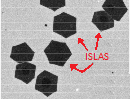
\includegraphics[width=.8\textwidth]{./imagenes/ejemplo1}
			\subcaption{}\label{ejemplo1}
		\end{subfigure}
		\begin{subfigure}[t]{2.5in}
			\centering
			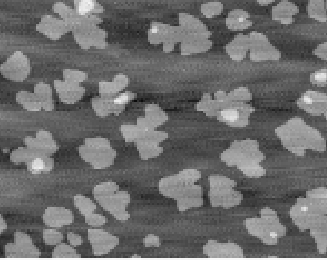
\includegraphics[width=.8\textwidth]{./imagenes/ejemplo2}
			\subcaption{}\label{ejemplo2}
		\end{subfigure}
		\begin{subfigure}[t]{2.5in}
			\centering
			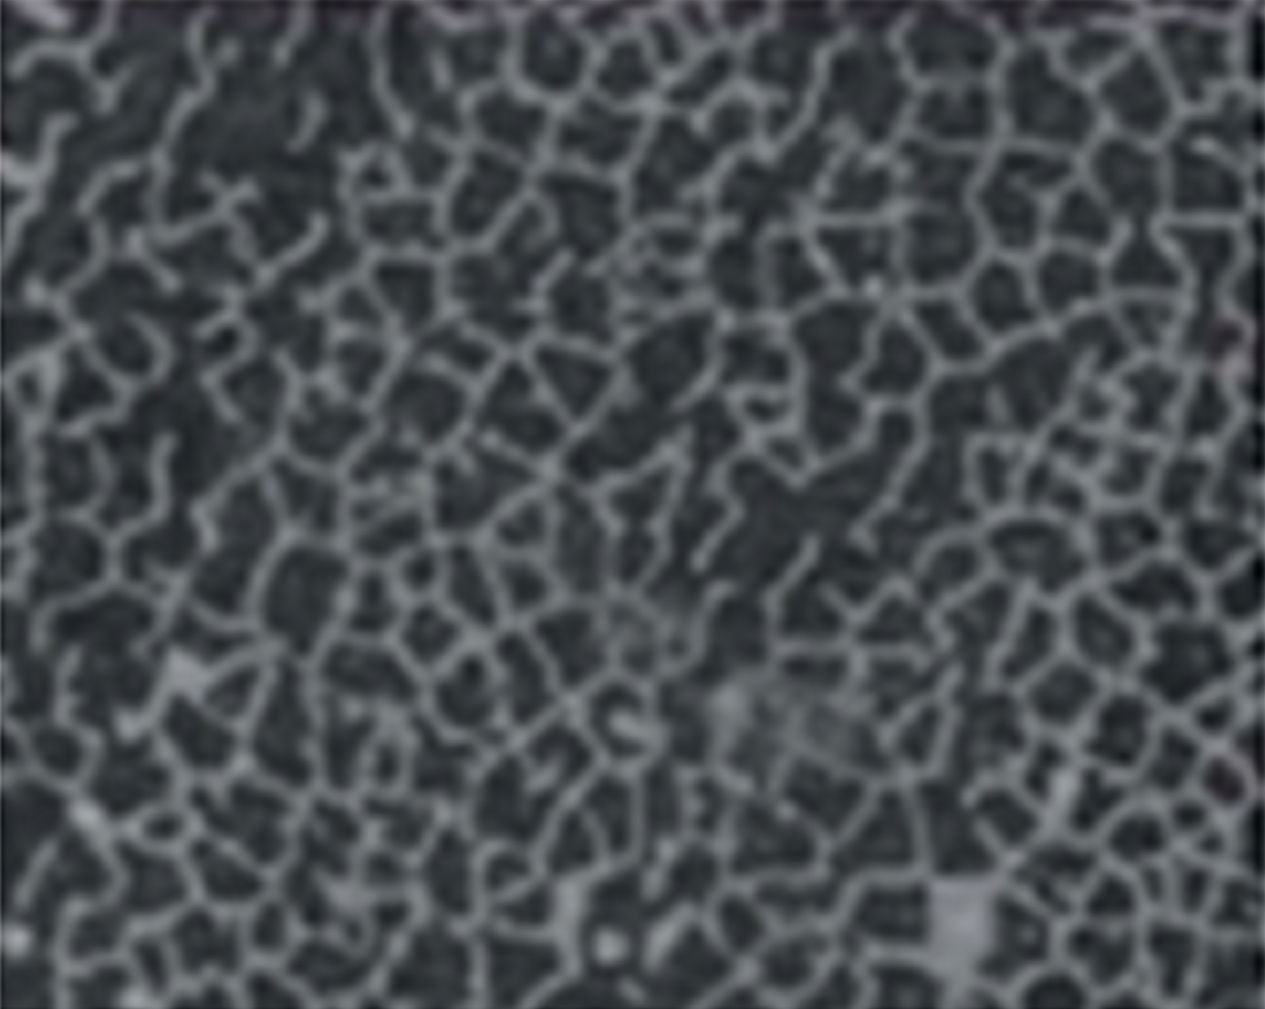
\includegraphics[width=.8\textwidth]{./imagenes/ejemplo3}
			\subcaption{}\label{ejemplo3}
		\end{subfigure}
		\begin{subfigure}[t]{2.5in}
			\centering
			
\includegraphics[width=.8\textwidth]{./imagenes/ejemplo4}
			\subcaption{}\label{ejemplo4}
		\end{subfigure}
	\end{center}
	\caption{Ejemplo de proyecciones en l\'{a}minas de materiales sintetizados mediante la deposici\'{o}n qu\'{i}mica de vapor}	
	\label{ejemploImagenes}
\end{figure}



